\documentclass[11pt]{article}
\usepackage{geometry, titlesec}
\usepackage[parfill]{parskip}
\usepackage[italicdiff]{physics}
\usepackage{amsfonts, amsthm, mathrsfs}
\usepackage[cm]{fullpage}
\usepackage{fancyhdr}
\usepackage{enumitem}
\usepackage{xcolor, soul}
\usepackage{siunitx, graphicx}
%\allowdisplaybreaks

\renewcommand{\thesubsection}{\thesection.\alph{subsection}}
\newcommand{\vfix}{\vspace{-\baselineskip}}

\makeatletter
\renewcommand*\env@cases[1][1.2]{%
  \let\@ifnextchar\new@ifnextchar
  \left\lbrace
  \def\arraystretch{#1}%
  \array{@{}l@{\quad}l@{}}%
}
\makeatother
 
\renewcommand{\footrulewidth}{.2pt}
%\setlist[enumerate]{leftmargin=*}
\pagestyle{fancy}
\fancyhf{}
\lhead{\textbf{Physics 323 Homework 1}}
\rhead{Lacey Rainbolt}
\setlength{\headheight}{11pt}
\setlength{\headsep}{11pt}
\setlength{\footskip}{24pt}
\lfoot{\today}
\rfoot{\thepage}

\titleformat{\section}[runin]{\normalfont\large\bfseries}{Problem \thesection.}{1em}{}
\titleformat{\subsection}[runin]{\normalfont\large\bfseries}{\thesubsection}{1em}{}
\titleformat{\subparagraph}[leftmargin]{\normalfont\normalsize\bfseries}{}{0pt}{}

\newcommand{\refeq}[1]{(\ref{#1})}

\newcommand{\beq}{\begin{equation*}}
\newcommand{\eeq}{\end{equation*}}

\newcommand{\beqn}{\begin{equation}}
\newcommand{\eeqn}{\end{equation}}

\newcommand{\blg}{\begin{align*}}
\newcommand{\elg}{\end{align*}}


\newenvironment{statement}[1]
{
	\section{#1}
	\color{darkgray}
	\ignorespaces
}

\newenvironment{problem}
{
	\subsection{}
	\color{darkgray}
	\ignorespaces
}

\newenvironment{solution}
{
	\paragraph{Solution.}
	\ignorespaces
}
{
    \bigskip
}

\DeclareSIUnit{\MeV}{\mega\electronvolt}
\DeclareSIUnit{\GeV}{\giga\electronvolt}

\begin{document}

\newcommand{\vq}{v_1}
\newcommand{\vw}{v_2}

\begin{statement}{(Jackson 11.3)}
	Show explicitly that two successive Lorentz transformations in the same direction are equivalent to a single Lorentz transformation with a velocity
	\beq
		v = \frac{\vq + \vw}{1 + \vq \vw / c^2}.
	\eeq
	This is an alternative way to derive the parallel-velocity addition law.
\end{statement}

\newcommand{\alp}{\alpha}
\newcommand{\bet}{\beta}
\newcommand{\gam}{\gamma}
\newcommand{\del}{\delta}
\newcommand{\lam}{\lambda}
\newcommand{\tht}{\theta}
\newcommand{\Lam}{\Lambda}
\newcommand{\Tht}{\Theta}

\newcommand{\Fab}{F^{\alp \bet}}
\newcommand{\Ua}{U^\alp}
\newcommand{\Usa}{U_\alp}
\newcommand{\Ub}{U^\bet}
\newcommand{\Xa}{X^\alp}
\newcommand{\Xsa}{X_\alp}
\newcommand{\Xb}{X^\bet}
\newcommand{\xap}{x^\alp_p}
\newcommand{\xaq}{x^\alp_q}

\begin{statement}{(Jackson 11.17)}
	The electric and magnetic fields \refeq{fields} of a charge in uniform motion can be obtained from Coulomb's law in the charge's rest frame and the fact that the field strength $\Fab$ is an antisymmetric tensor of rank 2 without considering \emph{explicitly} the Lorentz transformation.  The idea is the following.  For a charge in uniform motion the only relevant variables are the charge's 4-velocity $\Ua$ and the relative coordinate $\Xa = \xap - \xaq$, where $\xap$ and $\xaq$ aer the 4-vector coordinates of the observation point and the charge, respectively.  The only antisymmetric tensor that can be formed is $(\Xa \Ub - \Xb \Ua)$.  Thus the electromagnetic field $\Fab$ must be this tensor multiplied by some scalar function of the possible scalar products, $\Xsa \Xa$, $\Xsa \Ua$, $\Usa \Ua$.
\end{statement}

\newcommand{\vbb}{\vb{b}}
\newcommand{\vv}{\vb{v}}
\newcommand{\Eq}{E_1}
\newcommand{\Ew}{E_2}
\newcommand{\Be}{B_3}

\begin{figure}[b] \centering
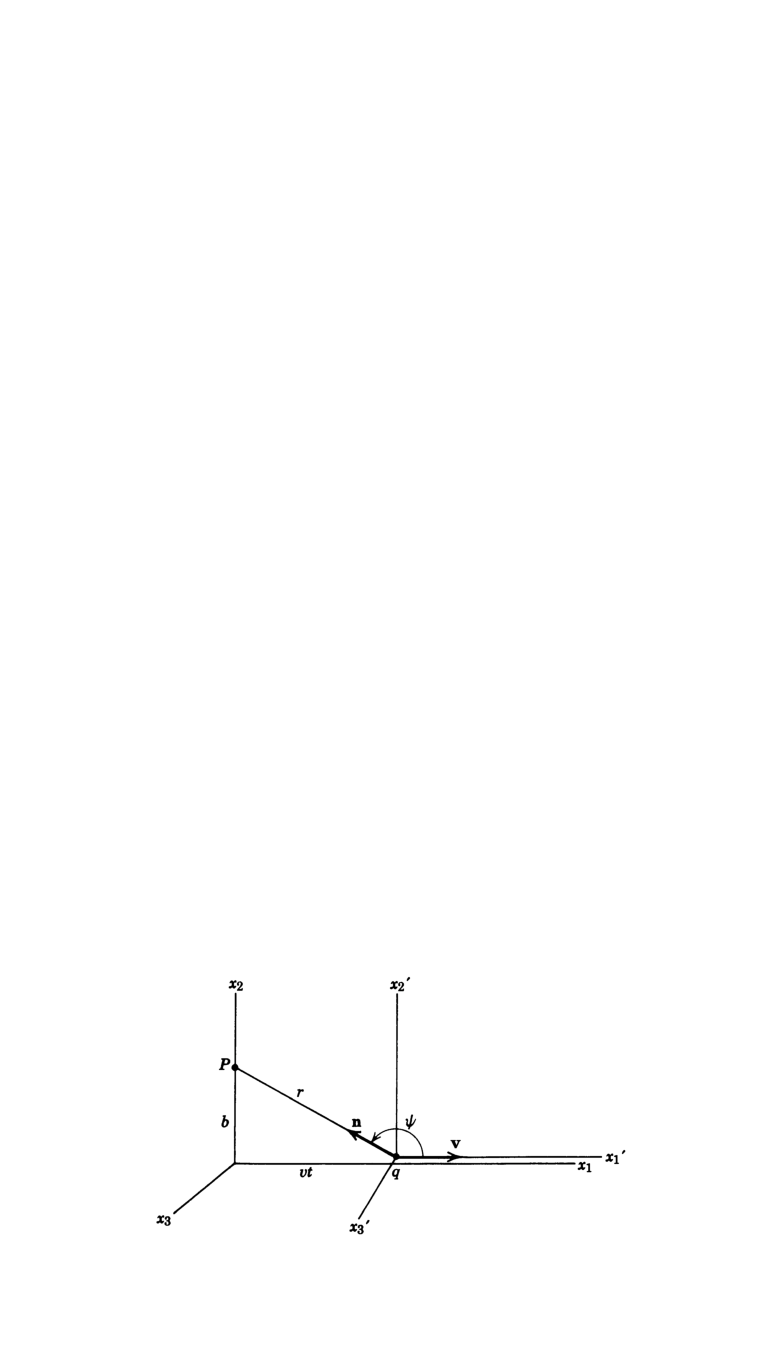
\includegraphics{11-8}
\caption{Particle of charge $q$ moving at constant velocity $\vv$ passes an observation point $P$ at impact parameter $b$.}
\label{11.8}
%\tag{11.8}
\end{figure}

\begin{problem} \label{2.a}
	For the geometry of Fig.~\ref{11.8} the coordinates of $P$ and $q$ at a common time in $K$ can be written $\xap = (ct, \vbb)$, $\xaq = (ct, \vv t)$, with $\vbb \vdot \vv = 0$.  By considering the general form of $\Fab$ in the rest frame of the charge, show that
	\beq
		\Fab = \frac{q}{c} \frac{\Xa \Ub - \Xb \Ua}{[(\Usa \Xa / c)^2 - \Xsa \Xa]^{3/2}}.
	\eeq
	Verify that this yields the expressions
	\begin{align} \label{fields}
		\Eq &= \Eq' = -\frac{q \gam v t}{(b^2 + \gam^2 v^2 t^2)^{3/2}}, &
		\Ew &= \gam \Ew' = \frac{\gam q b}{(b^2 + \gam^2 v^2 t^2)^{3/2}}, &
		\Be &= \gam \bet \Ew' = \bet \Ew,
	\end{align}
	with all other components vanishing, in the inertial frame $K$.
\end{problem}


\newcommand{\xpap}{{x'}^\alp_p}
\newcommand{\xpaq}{{x'}^\alp_q}
\newcommand{\Ya}{Y^\alp}
\newcommand{\Ysa}{Y_\alp}
\newcommand{\Yb}{Y^\bet}
\newcommand{\Ypa}{{Y'}^\alp}

\begin{problem}
	Repeat the calculation, using as the starting point the common-time coordinates in the rest fram, $\xpap = (ct', \vbb - \vv t')$ and $\xpaq = (ct', 0)$.  Show that
	\beq
		\Fab = \frac{q}{c} \frac{\Ya \Ub - \Yb \Ua}{(- \Ysa \Ya)^{3/2}},
	\eeq
	where $\Ypa = \xpap - \xpaq$.  Verify that the fields are the same as in \ref{2.a}.  Note that to obtain the results of \refeq{fields} it is necessary to use the time $t$ of the observation point $P$ in $K$ as the time parameter.
\end{problem}


\newcommand{\Za}{Z^\alp}
\newcommand{\Zsa}{Z_\alp}
\newcommand{\Zb}{Z^\bet}
\newcommand{\vbet}{\boldsymbol{\beta}}

\begin{problem}
	Finally, consider the coordinate $\xap = (ct, \vbb)$ and the ``retarded-time'' coordinate $\xaq = [ct - R, \vbet(ct - R)]$ where $R$ is the distance between $P$ and $q$ at the retarded time.  Define the difference as $\Za = [R, \vbb - \vbet(ct - R)]$.  Show that in terms of $\Za$ and $\Ua$ the field is
	\beq
		\Fab = \frac{q}{c} \frac{\Za \Ub - \Zb \Ua}{(\Usa \Za / c)^3}.
	\eeq
\end{problem}




\newcommand{\vr}{\vb{r}}
\newcommand{\vrperp}{\vr_\perp}

\begin{statement}{(Jackson 11.18)}
	The electric and magnetic fields of a particle of charge $q$ moving in a straight line with speed $v = \bet c$, given by \refeq{fields}, become more and more concentrated as $\bet \to 1$.  Choose axes so that the charge moves along the $z$ axis in the positive direction, passing the origin at $t = 0$.  Let the spatial coordinates of the observation point be $(x, y, z)$ and define the transverse vector $\vrperp$, with components $x$ and $y$.  Consider the fields and the source in the limit of $\bet = 1$.
\end{statement}

\newcommand{\rperp}{r_\perp}
\newcommand{\vE}{\vb{E}}
\newcommand{\vB}{\vb{B}}
\newcommand{\vh}{\vb{\hat{v}}}
\newcommand{\delctz}{\del(ct - z)}

\begin{problem} \label{3.a}
	Show that the fields can be written as
	\begin{align*}
		\vE &= 2q \frac{\vrperp}{\rperp^2} \delctz, &
		\vB &= 2q \frac{\vh \cross \vrperp}{\rperp^2} \delctz,
	\end{align*}
	where $\vh$ is a unit vector in the direction of the particle's velocity.
\end{problem}

\newcommand{\Ja}{J^\alp}
\newcommand{\valp}{v^\alp}

\begin{problem}
	Show that by substitution into the Maxwell equations that these fields are consistent with a 4-vector source density,
	\beq
		\Ja = q c \valp \del^2(\vrperp) \delctz,
	\eeq
	where the 4-vector $\valp = (1, \vh)$.
\end{problem}

\newcommand{\Ao}{A^0}
\newcommand{\Az}{A^z}
\newcommand{\vA}{\vb{A}}
\newcommand{\vAperp}{\vA_\perp}
\newcommand{\Thtctz}{\Tht(ct - z)}
\newcommand{\grperp}{\grad_\perp}

\begin{problem}
	Show that the fields of \refeq{3.a} are derivable from either of the following 4-vector potentials,
	\begin{align*}
		\Ao &= \Az = -2q \delctz \ln(\lam \rperp), &
		\vAperp &= 0,
	\end{align*}
	or
	
	\begin{align*}
		\Ao &= 0 = \Az, &
		\vAperp &= -2q \Thtctz \grperp \ln(\lam \rperp),
	\end{align*}
	where $\lam$ is an irrelevant parameter setting the scale of the logarithm.
	
	Show that the two potentials differ by a gauge transformation and find the gauge function, $\chi$.
\end{problem}




\newcommand{\mq}{m_1}
\newcommand{\mw}{m_2}
\newcommand{\pq}{p_1}
\newcommand{\pw}{p_2}

\begin{statement}{(Jackson 11.20)}
	The lambda particle ($\Lam$) is a neutral baryon of mass $M = \SI{1115}{\MeV}$ that decays with a lifetime of $\tau = \SI{2.9e-10}{\second}$ into a nucleon of mass $\mq \approx \SI{939}{\MeV}$ and a pi-meson of mass $\mw \approx \SI{140}{\MeV}$.  It was first observed in flight by its charged decay mode $\Lam \to p + \pi^-$ in cloud chambers.  The charged tracks originate from a single point and have the appearance of an inverted vee or lambda.  The particles' identities and momenta can be inferred from their ranges and curvature in the magnetic field of the chamber.
\end{statement}

\begin{problem}
	Using conservation of momentum and energy and the invariance of scalar products of 4-vectors show that, if the opening angle $\tht$ between the two tracks is measured, the mass of the decaying particle can be found from the formula
	\beq
		M^2 = \mq^2 + \mw^2 + 2 \Eq \Ew - 2 \pq \pw \cos\tht,
	\eeq
	where here $\pq$ and $\pw$ are the magnitudes of the 3-momenta.
\end{problem}

\begin{problem}
	A lambda particle is created with a total energy of \SI{10}{\GeV} in a collision in the top plate of a cloud chamber.  How far on the average will it travel in the chamber before decaying?  What range of opening angles will occur for a \SI{10}{\GeV} lambda if the decay is more or less isotropic in the lambda's rest frame?
\end{problem}




\begin{statement}{}
	Show that $\vE \vdot \vB$ is Lorentz invariant.  You can do this either by using the Lorentz transformation laws for $\vE$ and $\vB$ derived in class, or by writing $\vE \vdot \vB$ in a manifestly Lorentz invariant (and gauge invariant) form.
\end{statement}



\vfill
In addition to the course lecture notes, I consulted Jackson's \emph{Classical Electrodynamics} while writing these solutions.
\end{document}